\section{Real Data}
\label{sec:data}

We analyze a dataset that was collected to investigate the eating preferences of the wolf spider, genus \textit{Schizocosa}, towards the prey orders \textit{Diptera} and \textit{Collembola}.  Predators, collected in traps, had their gut-contents analyzed to determine whether or not the spiders ate any \textit{Diptera} or \textit{Collembola} within each time period.  The left panel of figure~\ref{fig:data} plots the percentage of spiders that had the prey in their guts across time.  Prey were similarly collected in traps distributed across the Berea College Forest in Madison County, Kentucky, USA.  These data were collected for each month from October $2011$ to March $2013$.  On average, $69$ spiders, and $111$ and $297$ \textit{Diptera} and \textit{Collembola}, respectively, were caught in each time period.  The range of the sample sizes, across all $18$ months is, $11$ to $181$ for caught spiders, from $7$ to $322$ for trapped \textit{Diptera}, and from $101$ to $755$ for trapped \textit{Collembola}.  The right panel of figure~\ref{fig:data} plots the total number of each order that was caught during each time period. 

\begin{figure}
  \centering
  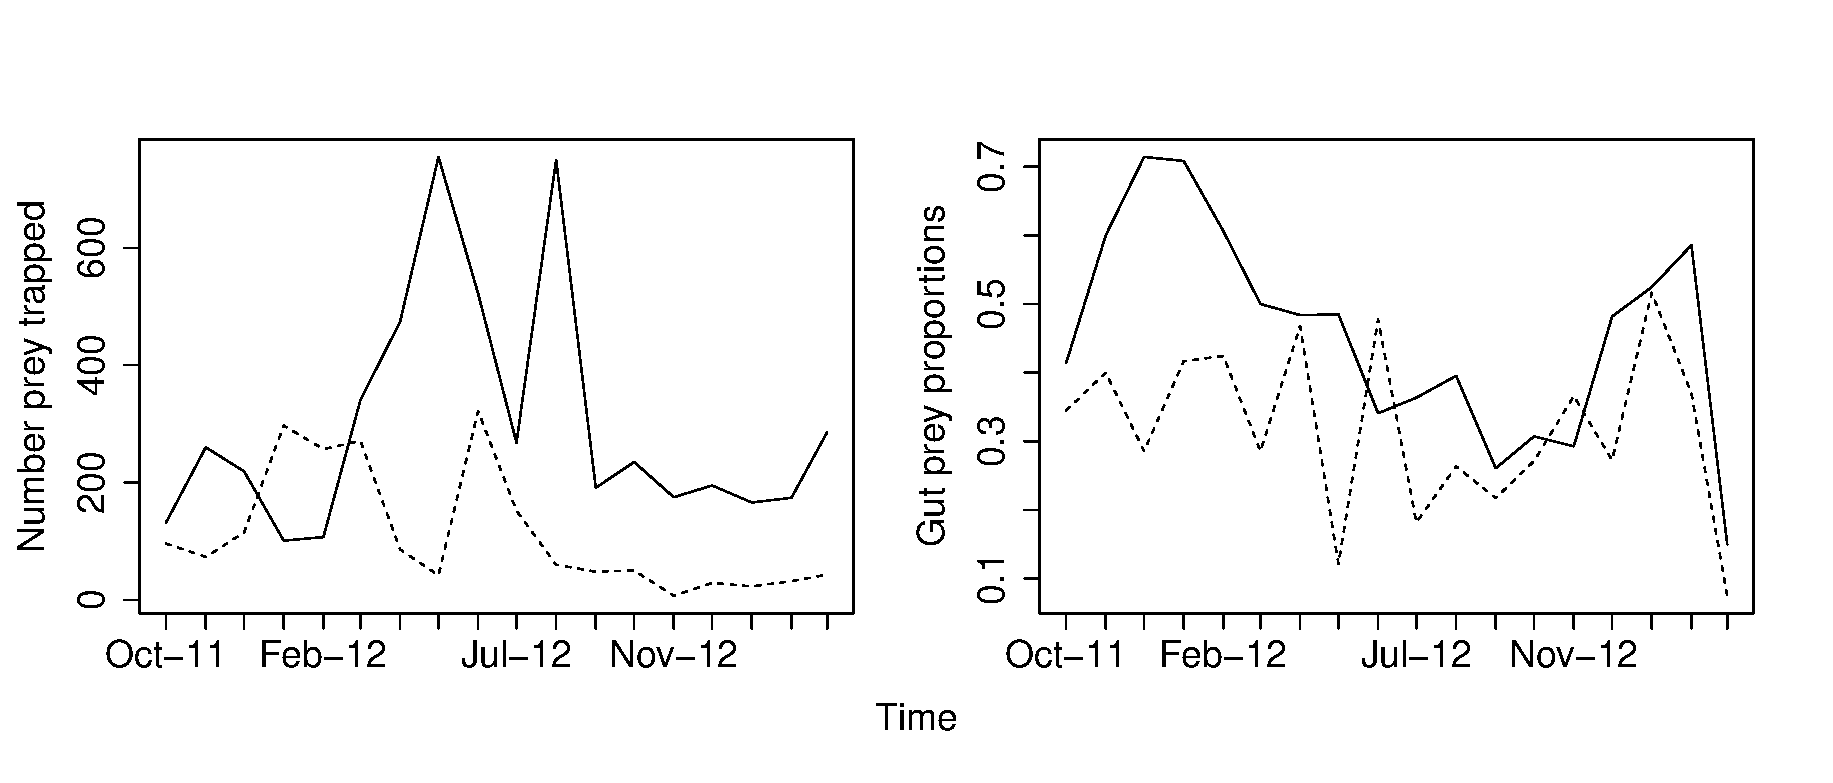
\includegraphics[scale=0.5]{data}
  \caption{For both \textit{Diptera} and \textit{Collembola}, the plots show the proportion of spiders with these orders found in their guts, and the number of these orders trapped in each time period.}
  \label{fig:data}
\end{figure}


These data provide an example of our hierarchy of hypotheses.  First, we test the model $c_{st} = c$ against $c_{st} = c_s$, to determine whether or not the wolf spider has different preferences for the two orders \textit{Diptera}  and \textit{Collembola}.  With, one degree of freedom, this likelihood ratio test indicates, $p-value < 0.0001$,  that two parameters, one for each order, fits these data better than one parameter for both.  Similarly, we test whether or not there is a significant effect across time by testing the model $c_{st} = c$ against $c_{st} = c_t$.  Here, the likelihood ratio test, with $17$ degrees of freedom, implies that the wolf spiders of the Berea College Forest eat these prey orders at different rates across the months of the year, $p-value < 0.0001$.  In fact, we find that the most parameter rich model, $\lambda_{st} = c_{st} \gamma_{st}$ fits these data best.  This model estimates $72$ parameters in total; since, in this case, there are two prey of interest and $18$ time periods, it takes $36$ parameters to estimate each $c_{st}$ and $\gamma_{st}$.  Figure~\ref{fig:cst} plots the point estimates and confidence intervals of $c_{st}$, for both prey across all time periods.  

\begin{figure}
  \centering
  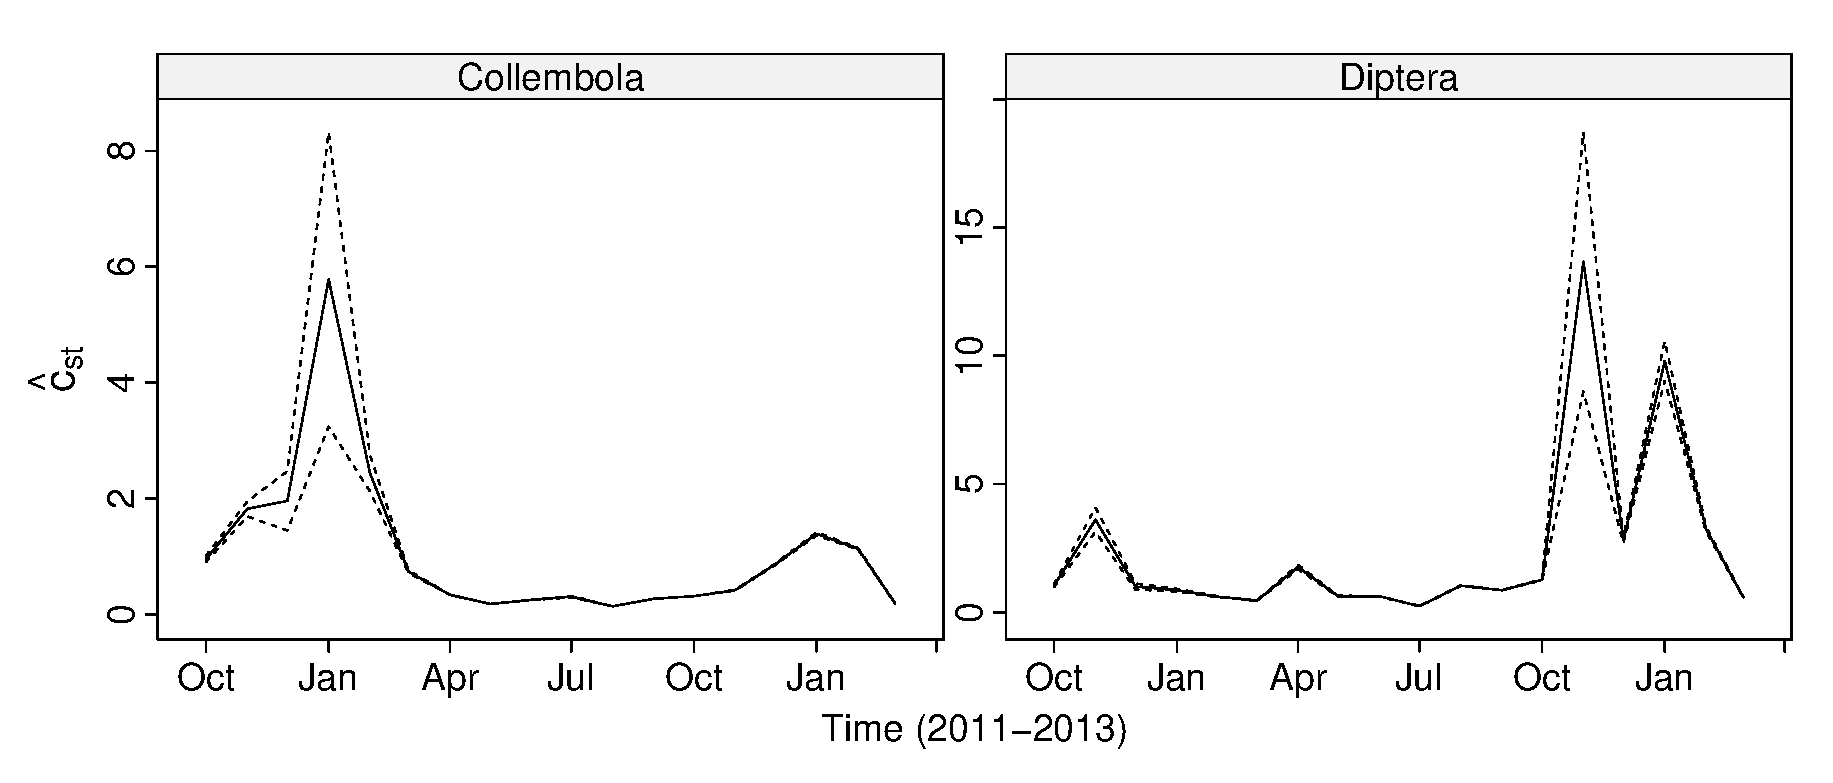
\includegraphics[scale=0.5]{cst}
  \caption{One plot for each prey order displays the point estimates and confidence intervals as estimated from the model $c_{st}$.}
  \label{fig:cst}
\end{figure}

With point estimates of $c_{st}$ under the model $\lambda_{st} = c_{st} \gamma_{st}$, we can test any number of linear contrasts.  For instance, consider $c_{1t} = c_{2t}$, for $t \in \{1, \ldots, 18\}$.  Using a level of significance of $0.05$, and after making a Bonferroni multiple comparisons adjustment, the data do not indicate that the two prey are differently preferred in October, November, and December of $2011$ and for March and July of $2012$.  


%%% Local Variables: 
%%% mode: latex
%%% TeX-master: "main"
%%% End: 
